\documentclass[lettersize,conference]{IEEEtran}
\usepackage{amsmath,amsfonts}
\usepackage{algorithmic}
\usepackage{algorithm}
\usepackage{array}
\usepackage[caption=false,font=normalsize,labelfont=sf,textfont=sf]{subfig}
\usepackage{textcomp}
\usepackage{stfloats}
\usepackage{url}
\usepackage{verbatim}
\usepackage{graphicx}
\usepackage{cite}

\begin{document}

\title{ECSE 425 Final Project\\Proposal for the Bonus Optimisation}

\author{
\IEEEauthorblockN{Amine Mallek}
\IEEEauthorblockA{\textit{ECSE Department} \\
\textit{McGill University}\\
Montreal, Canada \\
amine.mallek@mail.mcgill.ca}
\and
\IEEEauthorblockN{Bowen Cui}
\IEEEauthorblockA{\textit{ECSE Department} \\
\textit{McGill University}\\
Montreal, Canada \\
bowen.cui@mail.mcgill.ca}
\and
\IEEEauthorblockN{Kaan Gure}
\IEEEauthorblockA{\textit{ECSE Department} \\
\textit{McGill University}\\
Montreal, Canada \\
kaan.gure@mail.mcgill.ca}
\and
\IEEEauthorblockN{James Willems}
\IEEEauthorblockA{\textit{ECSE Department} \\
\textit{McGill University}\\
Montreal, Canada \\
james.willems@mail.mcgill.ca}
\and
\IEEEauthorblockN{Krishna Aroomoogon}
\IEEEauthorblockA{\textit{ECSE Department} \\
\textit{McGill University}\\
Montreal, Canada \\
krishna.aroomoogon@mail.mcgill.ca}
}

\maketitle

\begin{abstract}
This proposal outlines the general design of the proposed cache task for the optimisation of the final project.
\end{abstract}

\section{Introduction}
For our optimisation task, we have decided to implement a cache for out pipelined processor. The cache consists of two 4096-bit L1 caches for instruction and data respectively, and an arbiter to arbitrate the memory operations of the two L1 caches to the memory.\par
The L1 cache part of this task will be similar to the cache task from the mini-project 2. Since the performance of our processor will be assessed with simulations, multi-level caches would not be beneficial to the performance of our optimisation.
\subsection{Arbiter}
Since there is only one data bus in the unified memory, an arbiter will have to be implemented to schedule the memory accesses when there are two memory accesses from the two caches at the same time. The priority of the two requests is hard-coded in the simple arbiter, and the request from the data cache will always be accommodated first. Another function of the arbiter is that when a cache is fetching data from the memory, it will signal the pipeline to stall and wait for the memory access to finish. 

\section{Diagram}
\begin{figure}[H]
\centering
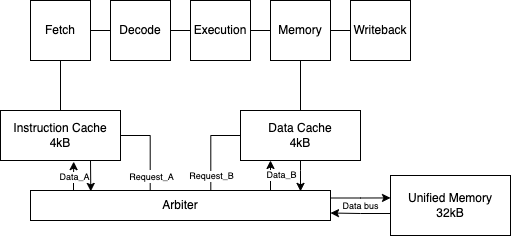
\includegraphics[width=2.5in]{cache_diagram}
\caption{The structure diagram of the cache subsystem.}
\label{fig_cache}
\end{figure}

\section{Performance Profiling}
To measure and compare the performance gain from the cache, we will measure the performance of the processor by running the same program in three different configurations. \par
The first configuration will be the bare processor without cache used, and the instruction memory and the data memory will be separate. In the second configuration, two 4096-bit L1 caches will be used for both instruction and data. In the third configuration, the sizes of the two caches will be increased to 8192 bits. \par
The code to generate the Fibonacci sequence will be used to measure the performance of the caches. The Fibonacci sequence is chosen because the speed on execution of the algorithm is dependent on fast memory accesses, and its pattern of memory accesses can fully take advantage of a data cache. The size of sequence generated will be set to a high value ($2000\sim3000$) to make sure that the performance difference between the three scenarios can be observed.\par

\end{document}


